\documentclass[chapter.computer_science.tex]{subfiles}
\begin{document}

\section{软件工程}
\subsection{概述}
结构化程序设计中,程序=算法+数据结构。软件工程中,软件=程序+文档。根据软件服务的对象范围不同可以将软件分为通用软件和定制软件,通用软件就例如操作系统、数据库软件等,定制软件则是为某一特定的需求所定制的软件。根据软件完成功能所处的层次不同,其又可以分为系统软件、中间件软件和应用软件。在这里着重说一下中间件软件,这是为了解决分布异构系统的集成问题而开发的软件,是{\bfseries 处于操作系统与应用软件中间的通用服务},具有标准的接口和协议。\\
软件工程起源在于软件危机,产生软件危机的原因在于第一、软件系统本身的复杂性,第二、软件开发的方法和技术不合理。软件工程就是要应用{\bfseries 系统化、规范化和定量}的方法来开发、运行和维护软件。其包含三个要素{\bfseries 方法、工具和过程}。\\
软件工程一般包括4个过程:软件规格说明(specification)、软件开发(development)、软件确认(validation)以及软件演进(evolution)。软件的生命周期又包含六个基本步骤,软件的生命周期模型又称为软件的过程模型:\\
\begin{enumerate}
    \item 制定计划:确定总目标,给出功能、性能、可靠性及{\bfseries 接口}等方面的要求,同时完成可行性评估、估计进度和可利用的资源。
    \item 需求分析:对需求给出详细的定义,编写需求说明书或系统功能说明书。
    \item 设计:又分为概要设计和详细设计,概要设计把各项需求转换成软件的体系结构,结构的每一部分都是意义明确的模块(划分模块)。详细设计为每个模块进行具体的描述(描述模块)。
    \item 程序编码。
    \item 测试:又分为单元测试、组装测试和有效性测试。单元测试针对模块,组装测试是将已测试过的模块按一定顺序组装起来测试,有效性测试是测试已开发出来的软件是否合格,能否交付。
    \item 运行维护:又分为改正性维护(修bug)、适应性维护(适应运行环境的变化)以及完善性维护(增强软件的功能)。
\end{enumerate}
\subsection{软件生命周期模型}
\subsubsection{瀑布模型}
\begin{figure}[H]
    \centering
    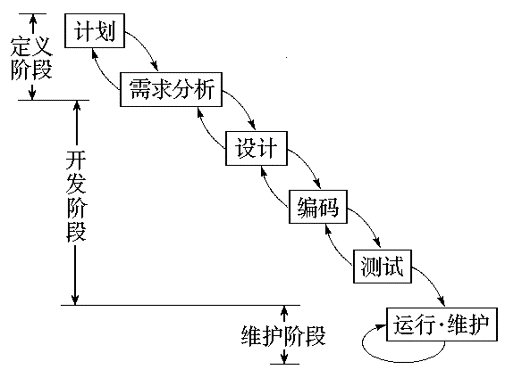
\includegraphics[scale=0.5]{./images/0032.png}
    \caption{瀑布模型}
\end{figure}
特点就是本活动的工作对象来源于上一活动的输出,这一输出往往是上一活动结束时里程碑式的文档。优点是降低了软件开发的复杂度,强调在软件实现之前必须进行分析和设计工作,以项目的阶段评审和文档控制为手段有效地对整个开发过程进行指导,保证了阶段间的正确衔接,能够及时发现并纠正开发中的缺陷。缺点是模型缺乏灵活性,无法解决需求不明确的问题且模型的风险控制能力较弱,整个活动是由文档驱动的,如果阶段间规定了过多的文档的话,会极大地增加系统的工作量。
\subsubsection{原型方法}
原型方法就是获得用户需求后,快速搭建一个原型系统,用户使用原型系统后提出修改的意见,使得需求尽可能地准确,这主要适用于在开发的早期,用户往往对系统只有一个模糊的想法,很难完全准确地表达系统的全面要求。原型方法有助于增进软件开发人员对用户系统服务需求的理解,可以更快速地确认产品的可行性。但这{\bfseries 较难作用于一个大型系统},对于一个大型系统来说,如果不经过系统分析得到系统的整体划分,直接使用原型来模拟是很困难的。而且{\bfseries 对于大量运算、逻辑性强的程序模块很难构造原型}。使用原型方法很容易忽略文档的构建,而且项目难以规划和管理。其{\bfseries 适用于联机事务处理系统,不适用于批处理系统}。\\
\subsubsection{演化模型}
演化模型下要进行2次软件开发,第一次是试验开发,得到原型产品用于探索可行性,弄清软件需求,第二次是在此基础上获得较为满意的软件产品。演化模型{\bfseries 适用于需求不清楚且开发周期短的中小型系统开发}。
\subsubsection{增量模型}
先对系统最核心或者需求最清晰的组件进行开发,然后再按优先级逐步对后续的需求进行开发,逐渐形成一个完整系统。这种方法{\bfseries 提高了系统的可靠性、稳定性和可维护性}。增量模型的缺点是{\bfseries 增量粒度难以选择且确定所有基本业务服务比较困难}。
\subsubsection{螺旋模型}
\begin{figure}[H]
    \centering
    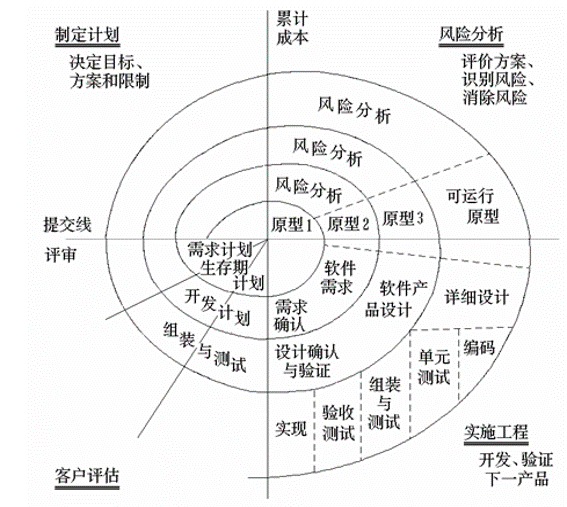
\includegraphics[scale=0.5]{./images/0033.png}
    \caption{螺旋模型}
\end{figure}
针对大型软件的开发,此方法{\bfseries 最大的特点就是引入了明确的风险管理}。每开发出一个原型时都要交由客户使用并进行反馈,然后决定是否进入螺旋线的下一个回路。
\subsubsection{喷泉模型(迭代模型)}
也称为迭代模型,该模型在各个开发阶段都没有特定的次序要求,可以并行进行,{\bfseries 可以在某个开发阶段中随时补充其他任何开发阶段遗漏的需求}。此方法提高了开发效率,缩短了开发周期,但缺点是难于管理。
\subsubsection{构件组装模型}
利用模块化的思想将整个系统模块化,然后在构件模型的支持下复用构件库中的一个或多个软件构件。此方法充分利用了软件复用,提高了开发效率,但缺乏通用的构件组装结构标准,风险较大且构件可重用性与系统高效性之间不易协调。
\subsubsection{快速应用开发(RAD)模型}
强调快速开发软件,极短的开发周期,此方法{\bfseries 适用于管理信息系统的开发}。而且如果一个应用不能被模块化,那就无法快速获取构造应用的构件。这种方法实质上就是将一个软件分为多个独立的模块,然后由若干个小组分别开发、测试这些模块,最后将其组装。
\subsubsection{统一过程模型(RUP)}
RUP模型{\bfseries 融合了喷泉模型和增量模型},将软件的生命周期分为4个阶段:初始阶段(Inception)、细化阶段(Elaboration)、构造阶段(Construction)和交付阶段(Transition)。每一个阶段都结束于一个主要的里程碑,结束一个阶段时对项目进行一次评估,以确定这个阶段的目标是否得到满足,如果满足的话,就允许项目进入下一个阶段。\\
\begin{enumerate}
    \item 初始阶段:目标是建立商业案例,并确定项目的边界。商业案例包括验收规范、风险评估、所需资源估计以及阶段计划等。此阶段结束的里程碑是{\bfseries 生命周期目标里程碑}。
    \item 细化阶段:目标是分析问题领域,建立体系结构基础,编制项目计划。里程碑是{\bfseries 生命周期体系结构里程碑}。包括风险分析文档、软件体系结构基础、项目计划、{\bfseries 初始版本的用户手册}。
    \item 构造阶段:将需求开发出来并集成为产品,{\bfseries 所有功能被详细测试}。里程碑是{\bfseries 初始运行能力里程碑}。包括可以运行的软件产品、{\bfseries 用户手册}等。
    \item 移交阶段:重点是确保软件对最终用户可用。里程碑为{\bfseries 产品发布里程碑},此时要确认最终目标是否实现,是否应该开启下一个版本的开发。
\end{enumerate}
RUP模型的迭代计划是由{\bfseries 风险驱动的},高风险因素在前两个阶段就得到解决,及早降低了系统风险。同时每一个阶段结束时还有质量评审,保证了里程碑文档的质量。
\subsubsection{敏捷模型(AM)和极限编程(XP)}
这是对已有生命周期模型的一个补充,并不是一个说明性过程。其原则是:尽早和不断提交有价值的软件使客户满意,而且{\bfseries 即使到了开发后期也欢迎改变需求}。同时{\bfseries 极限编程(XP)}是敏捷模型的一个实现过程。

\subsection{软件复用的两种实现机制}
合成复用:构件是基础,将功能实现的具体细节封装在构建内部,对外提供接口。利用构件来构造软件系统,有较高的生产率和较短的开发周期。\\
生成复用:利用可复用的模式,通过生成程序产生一个新的应用程序或程序段(个人感觉就像搜狐快站这样的玩意)。

\subsection{系统需求及可行性分析}
计算机的系统工程中定义的{\bfseries 计算机系统是元素的集合和排列},这些元素被组织在一起,以便通过处理外部信息来完成某些预定的目标。系统元素往往就是软件、硬件、数据库等。系统分析的目标就是:{\bfseries 识别用户需求},进行技术分析并评价,然后将功能分配给系统元素,建立成本和进度限制,{\bfseries 生成系统规格说明}。{\bfseries 系统分析和可行性分析的目标是明确系统是否值得做},避免投资损失。影响的因素也很简单,时间、资源、成本利润和技术条件能力。{\bfseries 最高层的系统体系结构叫体系结构语境图ACD},定义了系统使用信息的外部生产者,以及系统消息的外部消费者。

\subsection{软件需求分析}
软件需求分析的对象是用户要求,任务是准确地定义新系统的目标,导出目标系统的逻辑模型。需求分析的原则是:问题的信息域必须被表示和理解,软件将完成的功能的必须被定义,软件的行为必须被表示,且分析过程应遵循自顶向下和逐层细化的原则。其分别对应的三元模型为:数据模型、功能模型和行为模型。{\bfseries 数据建模需要合理地表示问题的信息域},其中信息域又包含三个不同的数据和控制视图即:信息内容和关系(个体数据和控制对象)、信息流(数据和控制在系统中流动变化的方式)以及信息结构(数据和控制项的内部组织)。{\bfseries 功能模型即为如何处理信息和数据变换},即输入、处理和输出。{\bfseries 行为模型即软件对外界事件做出的反应}。其中获取用户需求时,用户又分为两种,第一种是客户,就是掏钱买软件的人,第二种是最终用户(End user),就是实际用你软件的人。分析完成后,撰写《软件需求规格说明书》,然后交由评审。

\subsection{结构化需求分析}
{\bfseries 数据字典是结构化需求分析模型的核心},其主要包含{\bfseries 用于数据建模的实体关系图(ER图)},主要用于描述数据对象间的关系。{\bfseries 用于功能建模的数据流图(DFD图)},用于描述数据流在系统中流动的过程。{\bfseries 用于行为建模的状态迁移图(STD图)},用于描述对外部事件的响应方式。\\
E-R图是最常用的用来表示数据模型的方法,E-R图中的实体与属性用一个带名字的矩形来表示,上部表示实体名称,下面表示实体属性,用下划线标识实体的关键字属性。关系用连接实体的连线表示,连线上标出关系的名称,基数用连线的不同端点符号标识。\\
\begin{figure}
    \centering
    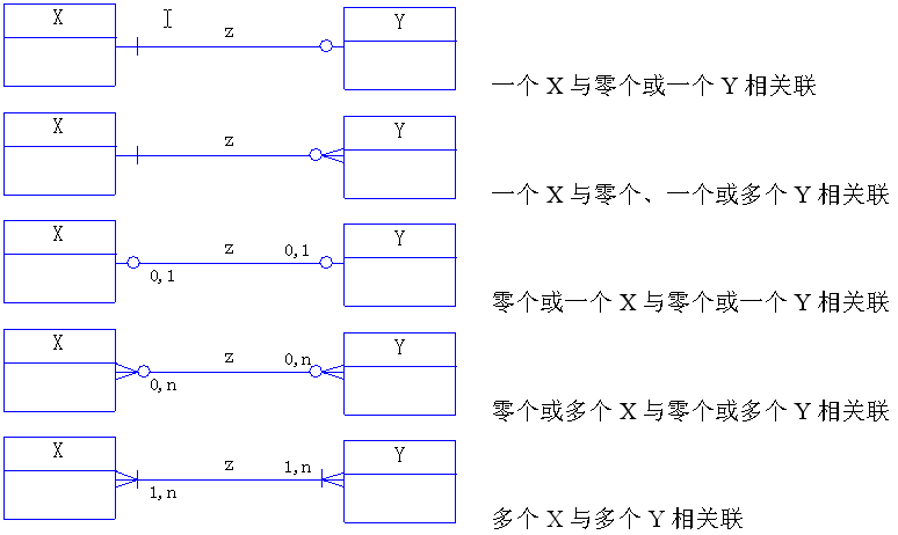
\includegraphics[scale=0.5]{./images/0034.png}
    \caption{E-R图}
\end{figure}
数据流图是描述信息流和数据输入输出时被系统的功能变换的图形化工具,用于功能建模。如下图,数据流图有四种基本元素,用圆圈代表数据的加工(通常是一个动词短语,描述完成的是什么加工),方框代表外部实体(数据的输入来源和处理结果要送往何处),箭头用来代指数据流(传输数据的通道),两道横线代表数据存储(保存数据)。\\
\begin{figure}[H]
    \centering
    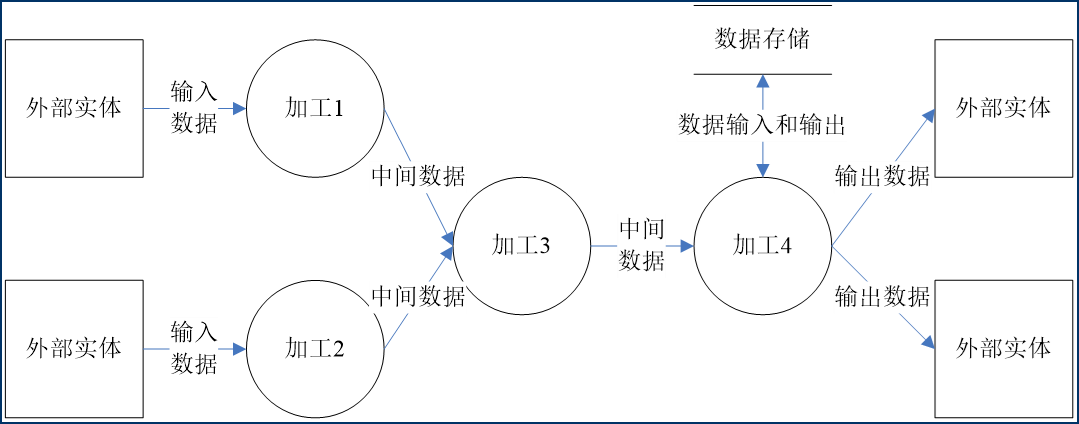
\includegraphics[scale=0.5]{./images/0035.png}
    \caption{数据流图}
\end{figure}
\begin{figure}[H]
    \centering
    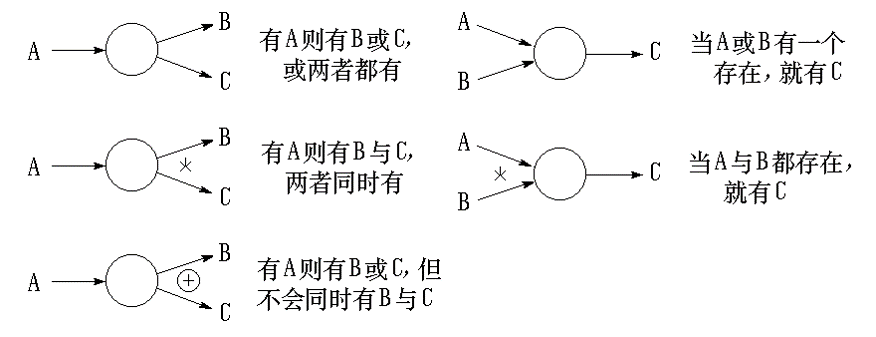
\includegraphics[scale=0.5]{./images/0036.png}
    \caption{数据流与加工的关系}
\end{figure}
数据词典用于对数据流图中出现的所有被命名的图形元素加以定义,使之有一个确切的解释。在写加工逻辑时,应注意对数据流图中的每一个基本加工,都必须有一个加工逻辑说明,而且要具体描述基本的加工是如何把输入数据流变成输出数据流的加工规则。可以使用判定表和判定树来处理加工时所需要依赖的逻辑条件的取值。\\
对于行为建模可以使用状态迁移图,状态迁移图用来描述系统或对象的状态,以及导致系统或对象状态改变的事件。在图中,用圆圈表示可得到的系统状态,用箭头表示从一种状态转移到另一种状态的迁移。


\end{document}
